\documentclass[11pt,a4paper]{article}
\usepackage[margin=1in]{geometry}
\usepackage{booktabs}
\usepackage{longtable}
\usepackage{array}
\usepackage{enumitem}
\usepackage{amsmath}
\usepackage{graphicx}
\usepackage{hyperref}
\usepackage{xcolor}
\usepackage{fancyhdr}
\usepackage{titlesec}
\usepackage[T1]{fontenc}
\usepackage{helvet}
\renewcommand{\familydefault}{\sfdefault}

\pagestyle{fancy}
\fancyhf{}
\fancyhead[L]{\small HLCL-001}
\fancyhead[R]{\small Rev 1}
\fancyfoot[C]{\thepage}

\newif\iffirstsection
\firstsectiontrue
\titleformat{\section}{\iffirstsection\global\firstsectionfalse\else\newpage\fi\large\bfseries}{\thesection}{1em}{}
\titleformat{\subsection}{\normalsize\bfseries}{\thesubsection}{1em}{}

\setlength{\parindent}{0pt}
\setlength{\parskip}{6pt}

\newcolumntype{L}[1]{>{\raggedright\arraybackslash}p{#1}}

\begin{document}

\begin{center}
{\LARGE\bfseries Humanity's Last Component Library --- EEE Component Standards}\\[6pt]
{\large (HLCL-001)}\\[4pt]
{\normalsize Rev 1 \quad---\quad \today}\\[4pt]
{\normalsize JD Brinton}
\end{center}

\vspace{12pt}

\tableofcontents

\section{Scope}

This document defines naming, parameter, and description conventions for all EEE components in the Humanity's Last Component Library (HLCL) Altium component library. All new components shall conform to these standards.

\section{General Rules}

\begin{enumerate}[nosep]
  \item Descriptions: ALL CAPS. No trailing period.
  \item Parameters stored as fields: Mixed case permitted (e.g.\ \texttt{10nF}, \texttt{+/-15\%}).
  \item SI prefixes: \texttt{p}, \texttt{n}, \texttt{u}, \texttt{m}, \texttt{k}, \texttt{M}. Never use $\mu$; use \texttt{u}.
  \item Units: \texttt{OHM} (descriptions), \texttt{V}, \texttt{A}, \texttt{W}, \texttt{Hz}, \texttt{F}, \texttt{H}.
  \item Tolerance: Absolute uses unit suffix (\texttt{+/-0.25pF}). Percentage uses \texttt{\%} (\texttt{5\%}). Never use $\pm$.
  \item Temperature range: hyphen-colon format, e.g.\ \texttt{-55:125}.
  \item Voltage: include \texttt{V} suffix, e.g.\ \texttt{25V}, \texttt{6.3V}.
  \item No Unicode. ASCII only in all database fields.
\end{enumerate}

\section{Altium Workspace Library Revision IDs}

Revision IDs in the Altium workspace library follow fixed patterns. The three-digit type code \texttt{xxx} identifies the component family. The complete allocation is listed with reference designator prefixes in Section~4.

\subsection{Components}

\begin{verbatim}
CMP-xxx-yyy-000000
\end{verbatim}

\begin{tabular}{@{}lL{11cm}@{}}
\toprule
Field & Definition \\
\midrule
\texttt{xxx} & Component type (three digits; allocation in Section~4). \\
\texttt{yyy} & Import series. Incremented each time a manufacturer or part series is imported so revision IDs do not collide with earlier imports of other series under the same type. \\
\texttt{000000} & Six-digit numeric suffix (unique per item within the \texttt{xxx}/\texttt{yyy} scope). \\
\bottomrule
\end{tabular}

\subsection{Component Templates}

\begin{verbatim}
CMPT-xxx
\end{verbatim}

\texttt{xxx} is the component type code (same as for components).

\subsection{Symbols}

\begin{verbatim}
SYM-xxx-000000
\end{verbatim}

\texttt{xxx} is the component type code. The final six digits are a numeric suffix as for components.

\subsection{Footprints}

\begin{verbatim}
PCC-xxx-000000
\end{verbatim}

\texttt{xxx} is the component type code. The final six digits are a numeric suffix as for components.

\section{Reference Designator Prefixes}

\begin{tabular}{@{}lll@{}}
\toprule
Prefix & Type code (\texttt{xxx}) & Component Type \\
\midrule
R & \texttt{000} & Resistor \\
C & \texttt{001} & Capacitor \\
U & \texttt{002} & Integrated Circuit \\
D & \texttt{003} & Diode \\
J & \texttt{004} & Connector \\
Q & \texttt{005} & Transistor \\
S & \texttt{006} & Switch \\
Y & \texttt{007} & Crystal Resonator (does not include oscillators) \\
I & \texttt{008} & Inductor \\
FB & \texttt{009} & Ferrite Bead \\
M & \texttt{010} & Mechanical (e.g.\ mounting holes, spacers) \\
\bottomrule
\end{tabular}

\section{Schematic Symbols}

One generic symbol per designator type. Symbol name equals the designator prefix or a functional variant.

\begin{tabular}{@{}lL{9cm}@{}}
\toprule
Symbol & Usage \\
\midrule
\texttt{CAP}  & All capacitors (C) \\
\texttt{RES}  & All resistors (R) \\
\texttt{IND}  & Inductors (I) \\
\texttt{FERRITE} & Ferrite beads (FB) \\
\texttt{LED}  & LEDs (D) \\
\texttt{DIODE} & All other diodes (D) \\
\texttt{NMOS} / \texttt{PMOS} & MOSFETs (Q) \\
\texttt{NPN} / \texttt{PNP} & BJTs (Q) \\
\texttt{SW}   & Switches (S) \\
\texttt{XTAL} & Crystals (Y) \\
\midrule
\multicolumn{2}{@{}l}{U and J: one symbol per unique part (pin-specific).} \\
\bottomrule
\end{tabular}

\section{Footprint Naming}

All footprints follow IPC-7351B naming.

\subsection{Two-Terminal Passives (C, R, I, FB)}

\begin{verbatim}
{TYPE}{LLWW}X{HH}{D}
\end{verbatim}

\begin{tabular}{@{}lL{10cm}@{}}
\toprule
Field & Definition \\
\midrule
\texttt{TYPE} & \texttt{CAPC} (capacitor chip), \texttt{RESC} (resistor chip), or \texttt{INDC} (inductor or ferrite bead chip) \\
\texttt{LLWW} & Body length and width in metric, each 2 digits $\times$ 0.1\,mm \\
\texttt{HH}   & Max component height in 0.01\,mm units, trailing zeros dropped \\
\texttt{D}    & Density: \texttt{N} (nominal), \texttt{L} (least), \texttt{M} (most) \\
\bottomrule
\end{tabular}

Examples: \texttt{RESC2012X06N}, \texttt{CAPC1005X05L}, \texttt{CAPC3225X25M}, \texttt{INDC1608X24N}.

\subsection{Semiconductors, Connectors, Crystals, Switches (U, D, J, Q, S, Y)}

Use the manufacturer package name or IPC-7351B land pattern name. Include pin count where applicable.

Examples: \texttt{SOT-23-3}, \texttt{QFN-48\_7X7}, \texttt{HC49}, \texttt{USB-C-16}.

\section{Description Format}

Descriptions are a single line, ALL CAPS, space-delimited, with fields ordered as defined per component type.

\subsection{Capacitors (C)}

\begin{verbatim}
CAPACITOR CERAMIC {VALUE} {TOLERANCE} {VOLTAGE} {DIELECTRIC} {EIA_SIZE}
\end{verbatim}

Example: \texttt{CAPACITOR CERAMIC 100NF 10\% 16V X7R 0402}

Capacitance values in descriptions are ALL CAPS:

\begin{tabular}{@{}ll@{}}
\toprule
Range & Format \\
\midrule
$< 1\,\text{nF}$ & \texttt{PF}: \texttt{100PF}, \texttt{4.7PF} \\
$1\,\text{nF} \leq C < 1\,\mu\text{F}$ & \texttt{NF}: \texttt{10NF}, \texttt{470NF} \\
$\geq 1\,\mu\text{F}$ & \texttt{UF}: \texttt{1UF}, \texttt{100UF} \\
\bottomrule
\end{tabular}

\subsection{Resistors (R)}

\begin{verbatim}
RESISTOR THICK FILM {VALUE} OHM {TOLERANCE} {EIA_SIZE}
\end{verbatim}

Example: \texttt{RESISTOR THICK FILM 10K OHM 1\% 0402}

For jumpers:
\begin{verbatim}
RESISTOR JUMPER 0 OHM {EIA_SIZE}
\end{verbatim}

Resistance values in descriptions use condensed ALL CAPS notation:

\begin{tabular}{@{}ll@{}}
\toprule
Range & Format \\
\midrule
$< 1\,\text{k}\Omega$ & Plain number: \texttt{100}, \texttt{4.7} \\
$1\,\text{k}\Omega \leq R < 1\,\text{M}\Omega$ & \texttt{K} suffix: \texttt{1K}, \texttt{47K}, \texttt{4.7K} \\
$\geq 1\,\text{M}\Omega$ & \texttt{M} suffix: \texttt{1M}, \texttt{2.2M} \\
\bottomrule
\end{tabular}

\subsection{Inductors (I)}

\begin{verbatim}
INDUCTOR {CONSTRUCTION} {VALUE} {TOLERANCE} {DCR} {EIA_SIZE}
\end{verbatim}

Example: \texttt{INDUCTOR MULTILAYER 4.7UH 20\% 0.1 OHM 0402}

Inductance values in descriptions use the unit suffix, ALL CAPS: \texttt{NH}, \texttt{UH}, or \texttt{MH} (e.g.\ \texttt{100NH}, \texttt{4.7UH}, \texttt{10MH}).

\subsection{Ferrite Beads (FB)}

\begin{verbatim}
FERRITE BEAD {IMPEDANCE} {RATED_CURRENT} {EIA_SIZE}
\end{verbatim}

\texttt{IMPEDANCE} is the typical impedance at 100\,MHz, numeric with the \texttt{OHM} unit (e.g.\ \texttt{120 OHM}, \texttt{1K OHM}).

Example: \texttt{FERRITE BEAD 60 OHM 1A 0402}

\subsection{Integrated Circuits (U)}

\begin{verbatim}
IC {FUNCTION} {KEY_SPEC} {PACKAGE}
\end{verbatim}

Example: \texttt{IC LDO REGULATOR 3.3V 500MA SOT-23-5}

\subsection{Diodes (D)}

\begin{verbatim}
DIODE {TYPE} {VOLTAGE} {CURRENT} {PACKAGE}
\end{verbatim}

Type keywords: \texttt{SCHOTTKY}, \texttt{ZENER}, \texttt{TVS}, \texttt{LED}, \texttt{RECTIFIER}, \texttt{ESD}.

Example: \texttt{DIODE SCHOTTKY 40V 1A SOD-123}

\subsection{Connectors (J)}

\begin{verbatim}
CONNECTOR {TYPE} {PIN_COUNT}P {PITCH} {ORIENTATION}
\end{verbatim}

Example: \texttt{CONNECTOR HEADER 10P 2.54MM VERTICAL}

\subsection{Transistors (Q)}

\begin{verbatim}
{TYPE} {POLARITY} {VOLTAGE} {CURRENT} {PACKAGE}
\end{verbatim}

Type keywords: \texttt{MOSFET}, \texttt{BJT}, \texttt{JFET}.

Example: \texttt{MOSFET N-CH 30V 5.8A SOT-23}

\subsection{Switches (S)}

\begin{verbatim}
SWITCH {TYPE} {CONFIGURATION} {RATING} {PACKAGE}
\end{verbatim}

Example: \texttt{SWITCH TACTILE SPST 50MA 12V SMD}

\subsection{Crystals (Y)}

\begin{verbatim}
CRYSTAL {FREQUENCY} {TOLERANCE} {CL} {PACKAGE}
\end{verbatim}

Example: \texttt{CRYSTAL 16MHZ +/-20PPM 12PF HC49}

\subsection{Mechanical (M)}

\begin{verbatim}
{CATEGORY} {DIMENSIONS} {ATTRIBUTES} {PACKAGE}
\end{verbatim}

CATEGORY and detail tokens are ALL CAPS. Type keywords:

\texttt{MOUNTING HOLE}, \texttt{SPACER}, \texttt{STANDOFF}, \texttt{FIDUCIAL}, \texttt{HARDWARE} (e.g.\ screws, standoffs, clips---use specific attributes).

Examples: \texttt{MOUNTING HOLE 2.1MM PTH}, \texttt{MECHANICAL MOUNTING HOLE 2.1MM NPTH}

\section{Database Fields}

\subsection{Common Fields (All Types)}

Present in every component database table.

\begin{longtable}{@{}llL{7.5cm}@{}}
\toprule
Column & Key? & Content \\
\midrule
\endhead
\texttt{Comment}          & PK & Full MPN. Unique key. \\
\texttt{Description}      &    & Per Section~7 format. \\
\texttt{MFG}              &    & Manufacturer name, ALL CAPS. \\
\texttt{MPN}              &    & Same as Comment. \\
\texttt{Package}          &    & Imperial (inch) standard package name, ALL CAPS. \\
\texttt{Library Path}     &    & SchLib filename. \\
\texttt{Library Ref}      &    & Symbol name (e.g.\ \texttt{CAP}, \texttt{RES}). \\
\texttt{Footprint Path}   &    & PcbLib filename. \\
\texttt{Footprint Ref}    &    & Footprint name, Nominal density. \\
\texttt{Footprint Path 2} &    & PcbLib filename (same). \\
\texttt{Footprint Ref 2}  &    & Footprint name, Least density. \\
\texttt{Footprint Path 3} &    & PcbLib filename (same). \\
\texttt{Footprint Ref 3}  &    & Footprint name, Most density. \\
\texttt{Qual}             &    & Qualification (e.g.\ \texttt{AEC-Q200}, blank if none). \\
\bottomrule
\end{longtable}

\subsection{Capacitors (C)}

\begin{tabular}{@{}lL{9cm}@{}}
\toprule
Column & Content \\
\midrule
\texttt{Value}     & Capacitance: \texttt{\{number\}\{prefix\}F} (e.g.\ \texttt{100pF}, \texttt{4.7nF}, \texttt{10uF}). \\
\texttt{Tolerance} & e.g.\ \texttt{5\%}, \texttt{+/-0.25pF}. \\
\texttt{Voltage}   & Rated DC voltage (e.g.\ \texttt{25V}). \\
\texttt{Tcr}       & Temperature characteristic (e.g.\ \texttt{+/-15\%}, \texttt{+/-30}). \\
\texttt{Tr}        & Operating temperature range (e.g.\ \texttt{-55:125}). \\
\bottomrule
\end{tabular}

\subsection{Resistors (R)}

\begin{tabular}{@{}lL{9cm}@{}}
\toprule
Column & Content \\
\midrule
\texttt{Value}     & Resistance: \texttt{\{number\}\{prefix\}}, no ``OHM'' (e.g.\ \texttt{100}, \texttt{4.7k}, \texttt{1M}). Jumpers: \texttt{0}. \\
\texttt{Tolerance} & e.g.\ \texttt{1\%}, \texttt{0.1\%}. \\
\texttt{Voltage}   & Limiting element voltage (e.g.\ \texttt{50V}). \\
\texttt{Tcr}       & Temperature coefficient (e.g.\ \texttt{+/-100}). Units: ppm/K implicit. \\
\texttt{Tr}        & Operating temperature range (e.g.\ \texttt{-55:155}). \\
\bottomrule
\end{tabular}

\subsection{Inductors (I)}

\begin{tabular}{@{}lL{9cm}@{}}
\toprule
Column & Content \\
\midrule
\texttt{Value}     & Inductance: \texttt{\{number\}\{prefix\}H} (e.g.\ \texttt{100nH}, \texttt{4.7uH}, \texttt{10mH}). \\
\texttt{Tolerance} & e.g.\ \texttt{5\%}, \texttt{20\%}. \\
\texttt{DCR}       & DC resistance (e.g.\ \texttt{0.1OHM}, \texttt{2.1mOHM}). \\
\texttt{Current}   & Rated current (RMS) or \texttt{Isat} as applicable (e.g.\ \texttt{1.5A}). \\
\texttt{Tr}        & Operating temperature range (e.g.\ \texttt{-40:85}). \\
\bottomrule
\end{tabular}

\subsection{Ferrite Beads (FB)}

\begin{tabular}{@{}lL{9cm}@{}}
\toprule
Column & Content \\
\midrule
\texttt{Value}     & Impedance at 100\,MHz, numeric with \texttt{OHM} (e.g.\ \texttt{60OHM}, \texttt{1KOHM}) unless another reference frequency is documented, then state it in the field. \\
\texttt{Current}   & Rated current (RMS) (e.g.\ \texttt{1A}, \texttt{2A}). \\
\texttt{DCR}       & DC resistance (e.g.\ \texttt{0.1OHM}). \\
\texttt{Tr}        & Operating temperature range (e.g.\ \texttt{-40:85}). \\
\bottomrule
\end{tabular}

\subsection{Integrated Circuits (U)}

\begin{tabular}{@{}lL{9cm}@{}}
\toprule
Column & Content \\
\midrule
\texttt{Tr}        & Operating temperature range (e.g.\ \texttt{-40:85}). \\
\bottomrule
\end{tabular}

\subsection{Diodes (D)}

\begin{tabular}{@{}lL{9cm}@{}}
\toprule
Column & Content \\
\midrule
\texttt{Vr}        & Reverse voltage or breakdown voltage (e.g.\ \texttt{40V}). \\
\texttt{Vf}        & Forward voltage drop (e.g.\ \texttt{0.45V}). \\
\texttt{Current}   & Forward current rating (e.g.\ \texttt{1A}). \\
\texttt{Tr}        & Operating temperature range (e.g.\ \texttt{-55:150}). \\
\bottomrule
\end{tabular}

\subsection{Connectors (J)}

\begin{tabular}{@{}lL{9cm}@{}}
\toprule
Column & Content \\
\midrule
\texttt{Current}   & Current rating per pin if applicable (e.g.\ \texttt{1A}). \\
\texttt{Voltage}   & Rated voltage if applicable. \\
\bottomrule
\end{tabular}

\subsection{Transistors (Q)}

\begin{tabular}{@{}lL{9cm}@{}}
\toprule
Column & Content \\
\midrule
\texttt{Voltage}   & $V_{DS}$ or $V_{CE}$ rating (e.g.\ \texttt{30V}). \\
\texttt{Current}   & $I_D$ or $I_C$ rating (e.g.\ \texttt{5.8A}). \\
\bottomrule
\end{tabular}

\subsection{Switches (S)}

\begin{tabular}{@{}lL{9cm}@{}}
\toprule
Column & Content \\
\midrule
\texttt{Voltage}   & Rated voltage (e.g.\ \texttt{12V}). \\
\texttt{Current}   & Rated current (e.g.\ \texttt{50mA}). \\
\bottomrule
\end{tabular}

\subsection{Crystals (Y)}

\begin{tabular}{@{}lL{9cm}@{}}
\toprule
Column & Content \\
\midrule
\texttt{Value}     & Frequency with unit (e.g.\ \texttt{16MHz}, \texttt{32.768kHz}). \\
\texttt{Tolerance} & Frequency tolerance (e.g.\ \texttt{+/-20ppm}). \\
\texttt{CL}        & Load capacitance (e.g.\ \texttt{12pF}). \\
\texttt{ESR}       & Equivalent series resistance (e.g.\ \texttt{40OHM}). \\
\texttt{Tr}        & Operating temperature range (e.g.\ \texttt{-40:85}). \\
\bottomrule
\end{tabular}

\subsection{Mechanical (M)}

\begin{tabular}{@{}lL{9cm}@{}}
\toprule
Column & Content \\
\midrule
none & none \\
\bottomrule
\end{tabular}

\section{Footprint Density Assignment}

Three IPC-7351B density levels are stored per component.

\begin{tabular}{@{}lll@{}}
\toprule
Slot & Suffix & IPC Density Level \\
\midrule
Footprint Ref   & \texttt{N} & Nominal (default) \\
Footprint Ref 2 & \texttt{L} & Least (tightest spacing) \\
Footprint Ref 3 & \texttt{M} & Most (largest pads) \\
\bottomrule
\end{tabular}

Semiconductors, connectors, switches, and crystals: populate Footprint Ref only. Leave slots 2 and 3 blank unless IPC density variants exist.

\section{Schematic Symbol Drawing Standards}

Use Altium default schematic editor settings. The following are called out explicitly to prevent deviation.

\begin{enumerate}[nosep]
  \item Grid: 100\,mil snap, 100\,mil visible.
  \item Pin length: 200\,mil default. May deviate to improve readability.
  \item Pin font: \textbf{Arial 8pt}.
  \item Line width: default (1px/small).
  \item Filled body for passives. Unfilled (outline only) for ICs.
  \item Designator visible, Value visible. Both use default font.
  \item No color overrides. Use Altium default pin/body/text colors.
  \item Pins shall snap to grid. All pin endpoints must land on 10mil grid.
  \item Pin numbers: always visible on all pins.
  \item Set pin Electrical Type (passive, input, output, power, etc.) when well defined in the component datasheet.
  \item Hidden pins are prohibited.
  \item Component symbol shall be centered on the origin of the symbol editor (as close as grid permits).
\end{enumerate}

\begin{figure}[h]
\centering
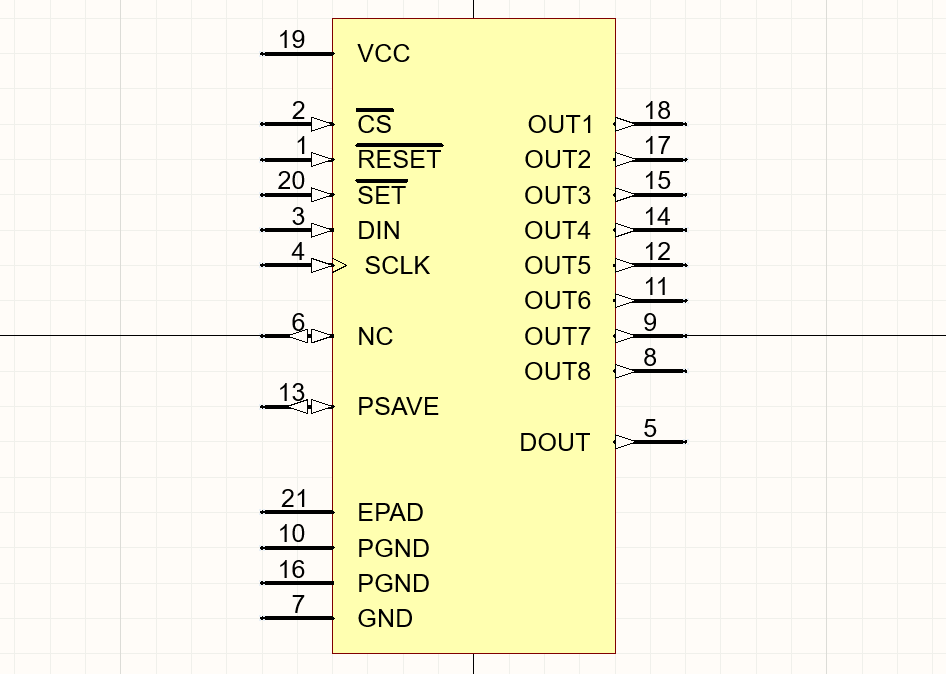
\includegraphics[width=0.6\textwidth]{example-symbol.png}
\caption{Example schematic symbol.}
\end{figure}

\section{PCB Footprint Drawing Standards}

Do not populate the footprint Description field. All authoritative component descriptions are stored in the component database templates and shall not be duplicated in footprints.

\subsection{Default Units}

The PcbLib's default display unit shall be millimetres. All dimensions in this section, in vendor data, and in the IPC-7351B math used by the autogenerator are in millimetres unless explicitly noted otherwise.

\subsection{Layer Usage}

\begin{tabular}{@{}lL{9cm}@{}}
\toprule
Layer & Content \\
\midrule
Top Layer        & Copper pads only. \\
Top Solder       & Solder mask openings (manual expansion, see below). \\
Top Paste        & Paste mask openings (rule-based, defined at PCB level). \\
Mechanical 1     & 3D body model. \\
Mechanical 15    & Component centroid (cross-hair) and component outline. \\
\bottomrule
\end{tabular}

Layers explicitly \textbf{not used} in footprints:

\begin{tabular}{@{}lL{9cm}@{}}
\toprule
Layer & Rationale \\
\midrule
Top Overlay (silkscreen) & No component outline on silkscreen. Silkscreen designators are added during layout, not in the footprint. \\
Courtyard (Mech 13/etc.) & Not used. Board-level clearance rules handle spacing. \\
\bottomrule
\end{tabular}

\subsection{Pads}

\begin{enumerate}[nosep]
  \item Shape: Rounded rectangle, 25\% corner radius (per IPC-7351B).
  \item Pad dimensions: per IPC-7351B calculator using manufacturer dimensions.
  \item Solder mask expansion: manual, set to 0.05\,mm (1.97\,mil) per pad.
  \item Paste mask expansion: not set per pad; use board-level rule.
  \item Minimum solder mask sliver between adjacent pads: 0.1\,mm. If IPC-calculated pads violate this, add solder mask to combine apertures.
  \item Thermal pad (exposed pad): include if specified by manufacturer. Paste mask subdivided per manufacturer recommendation.
\end{enumerate}

\subsection{3D Model (Mechanical 1)}

\begin{enumerate}[nosep]
  \item Two-terminal chip components (CAPC, RESC, INDC, FB) shall use the parametric STEP generator under \texttt{house/stepgen/} (pure-Python, no external CAD dependencies). Because the IPC-7351B density variants (L / N / M) only change the pad geometry --- not the component body --- the generator deduplicates by footprint root (FootprintName minus its trailing density letter) and emits one STEP file per unique body into \texttt{build/intermediate/step/<root>.step}, e.g. \texttt{build/intermediate/step/CAPC0402X20.step} is shared by \texttt{CAPC0402X20\{L,N,M\}}. The build pipeline embeds (zlib-compressed) the same STEP into all three density variants of each root in \texttt{build/output/house.PcbLib} so the library is standalone.
  \item Other components: use a manufacturer STEP file or, as a last resort, a simple extruded box matching L $\times$ W $\times$ H nominal.
  \item Model shall use nominal component dimensions from the manufacturer datasheet.
  \item Model origin shall align with footprint origin (component centroid).
  \item Model Z-offset: place directly on pad surface (Z = 0).
  \item Body colour conventions for autogenerated chip models:
    \begin{itemize}[nosep]
      \item CAPC -- MLCC tan / cream over silver (Sn) terminals. Body and terminals have rounded edges (cylindrical fillet $r = 0.05$\,mm, clamped to $\min(L,W,H)/4$).
      \item INDC, FB -- ferrite blue body over silver terminals. Same rounded-edge geometry as CAPC.
      \item RESC -- mid-grey alumina substrate, near-black passivation cover on top, slightly darker grey end-cap terminals. Sharp edges (no fillets). Each terminal is a "C" shape wrapping around the substrate (vertical end face + top strip + bottom strip), so the substrate is supported only by the bottom wraps and the passivation cover sits flush with the terminals' top wraps.
    \end{itemize}
\end{enumerate}

\subsection{Component Outline and Centroid (Mechanical 15)}

\begin{enumerate}[nosep]
  \item Line width: 0.1\,mm.
  \item Component outline: closed rectangle matching the 2D projection of the 3D body (nominal L $\times$ W).
  \item Centroid: cross-hair at component origin. Each arm shall be no longer than the corresponding half-extent of the component outline (so the cross never escapes the body rectangle), and shall be capped at 0.5\,mm per arm so the total cross length is at most 1\,mm regardless of body size.
\end{enumerate}

\subsection{Pin 1 Marking}

Required on all oriented parts (ICs, diodes, transistors, polarized capacitors, connectors with keying).
Not required on non-polarized two-terminal passives (standard capacitors, resistors, crystals).

\begin{enumerate}[nosep]
  \item Layer: Top Overlay.
  \item Content: single period character ``\texttt{.}'' (dot).
  \item Font: TrueType Arial, text height 2\,mm.
  \item Placement: adjacent to pin~1 pad, outside the component outline.
  \item The marker is a free text object (not locked to pad) so it may be repositioned during layout.
\end{enumerate}

\subsection{Footprint Origin}

\begin{enumerate}[nosep]
  \item Origin placed at the geometric centroid of the pad pattern.
  \item For symmetric packages: center of the body.
  \item For connectors: pin~1 or the mechanical datum specified by the manufacturer.
\end{enumerate}

\begin{figure}[h]
\centering
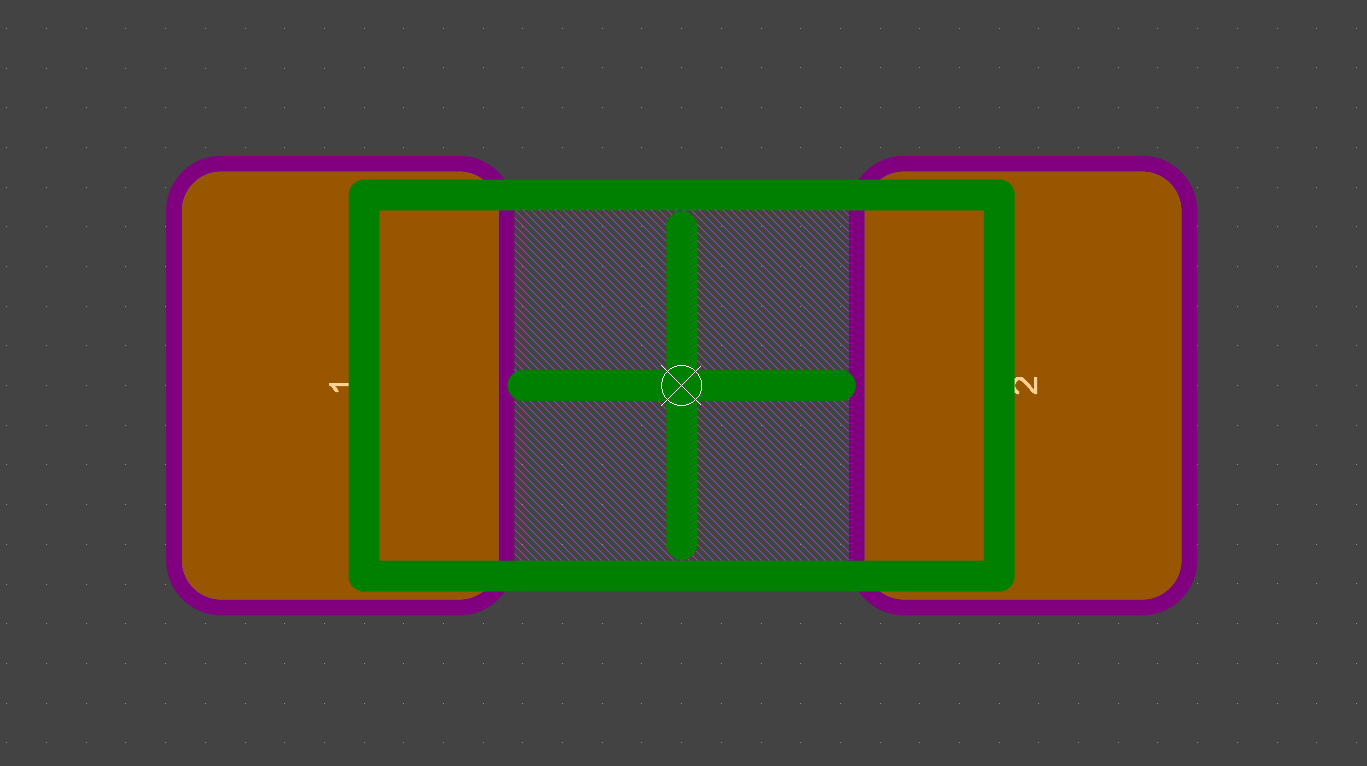
\includegraphics[width=0.6\textwidth]{example-footprint.png}
\caption{Example PCB footprint.}
\end{figure}

\end{document}
